\documentclass[a4paper]{jctart15b}

\oddsidemargin=-1.5mm \evensidemargin=-2.5mm

\usepackage[pdftex]{graphicx}
\usepackage{epstopdf}        %%% Пакеты для работы с рисунками (компиляция PDF/LaTeX) и др.
\usepackage{amsthm,amsfonts,amsmath,amssymb}

\usepackage{indentfirst}
\usepackage{color}
\usepackage{algorithmic}
\usepackage{algorithm}
\usepackage{float}
\usepackage{tikz}
\usepackage{tikz-qtree}

\begin{document}

\newtheorem{definition}{Определение}
\newtheorem{example}{Пример}

\newcommand{\fictAquantor}{\ensuremath{\forall\colon\varnothing}}
\newcommand{\fictEquantor}{\ensuremath{\exists\colon\varnothing}}
\newcommand{\bomega}{\boldsymbol{\omega}}
\newcommand{\bphi}{\boldsymbol{\phi}}
\newcommand{\eqdef}{\stackrel{\mathrm{df}}{=}}
\newcommand{\bigand}[2]{\raisebox{-2pt}{\ensuremath{\overset{#1}{\underset{#2}{\text{\Large\&\normalfont}}}}}}

\setcounter{page}{1}

\markboth{А.\,В.~Давыдов, А.\,А.~Ларионов, Е.\,А.~Черкашин}{Метод трансляции первопорядковых формул в позитивно-образованные формулы}

\title{Алгоритмы преобразования первопорядковых формул в позитивно-образованные формулы\let\thefootnote\relax\footnote{\copyright\ ИВТ СО РАН, 2016}}

\author{
{\sc А.\,В.~Давыдов${}^*$, А.\,А.~Ларионов, Е.\,А.~Черкашин}\\
\vtop{\small ФГБУН Институт динамики систем и теории управления имени В.\,М.~Матросова СО~РАН}\\
$^*$\vtop{\small Контактный e-mail: \tt artem@icc.ru}
}

\date{}
\maketitle

\begin{abstract}
  В статье приводится краткое описание языка позитивно"=образованных формул и
  рассматриваются вопросы их обработки перед запуском автоматических алгоритмов поиска вывода. Представлен новый метод преобразования формул языка исчисления предикатов в язык позитивно"=образованных формул, с сохранением исходной эвристической структуры знаний. Предложен упрощенный алгоритм для трансляции задач представленных на языке дизъюнктов в язык позитивно"=образованных формул. Приводятся результаты тестирования разработанного метода.

    {\it Ключевые слова}: математическая логика, автоматическое доказательство теорем, алгоритмы трансляции
\end{abstract}

\paragraph{Введение.}

Автоматическое доказательство теорем (АДТ) и его приложения активно развивается, что можно видеть из работ ежегодной конференции CADE - Conference on Automated Deduction (www.cadeinc.org). Например, каждый год на секции “System description” представляется новая система для АДТ (прувер), либо рассматривается развитие ранее разработанных известных систем.

В данной работе рассматривается логическое исчисление позитивно-образованных формул (ПОФ-исчисление) и построенный на его основе метод АДТ. ПОФ-исчисление выгодно отличается от возможностей других, логических, средств формализации предметной области и поиска логических выводов: выразительностью в сочетании с компактностью представления знаний, «естественным» параллелизмом их обработки, крупноблочностью и меньшей комбинаторной сложностью выводов, высокой совместимостью с эвристиками и б\'ольшими возможностями для интерактивного доказательства (interactive proof-search). В выделенном классе формул возможно построение конструктивного доказательства. Данный класс формул существенно шире класса хорновских дизъюнктов: на логическую формализацию аксиоматической базы предметной области не накладывается никаких ограничений, а целевое утверждение -- это конъюнкция запросов в смысле языка Пролог.

Исчисление ПОФ возникло в работах акаденика РАН С.\,Н.~Васильева и
А.\,К.~Жерлова \cite{SNV1990,ICDS2000} в результате описания и решения задач
теории управления. В \cite{ICDS2000} исчисление описывается как логический
формализм первого порядка, приводятся примеры описания и решения задач теории
управления, эффективно (с точки зрения выразительности языка и
производительности средств доказательств теорем) решенных с помощью исчисления ПОФ (например, управление группой лифтов, планирование действий мобильного робота и наведение телескопа), а также доказательства корректности и полноты исчисления (дальнейшее развитие исчисления представлено в \cite{jour2}).

В процессе разработки программной системы для АДТ \cite{mipro2013}, основанной на
исчислении ПОФ, проводится тестирование системы на задачах из библиотеки TPTP
(Thousands of Problems for Theorem Provers) \cite{tptp}. Формат, в котором
представлены задачи в TPTP, стал стандартом де-факто среди сообщества изучающего
автоматизацию рассуждений, например, в работе \cite{SMTtoTPTP}, рассматривается
программа-конвертер из формата SMT-LIB в фромат TPTP. Задачи, содержащиеся в
библиотеке, -- это первопорядковые логические теоремы, представленные в виде
набора формул. Формулы, в общем случае, распределены между различными файлами
(библиотеками формул), а также разделены на классы в зависимости от особенностей
их структуры:  FOL, CNF и др.

Для загрузки задач необходима разработка конфертера, позволяющего преобразовывать
формулы, представленные в формате TPTP, в структуры данных, которые принимет на
вход прувера.  Конвертер включает в себя транслятор задач, в формулы FOL, а
также процедуры преобразования FOL в формат ПОФ.

Задача конвертации неривиальна из-за особой структуры формул ПОФ-исчисления. В
данной работе предлагается эффективная методика трансляции и преобразования.  В
качестве критерия эффективности в данной работе понимается количество шагов
[ЧЕГО?] и размер получаемых формул -- количество кванторов и ветвлений в древовидном представлении ПОФ. Приводятся результаты тестирования разработанного метода, которые позволяют сделать вывод о том, что существует определенный класс первопорядковых формул, [не принимаемый во внимание существующими системами АДТ???], в то время как в ПОФ-исчислении для данного класса формул существуют специальные стратегии повышающие эффективность поиска вывода.

\paragraph{Предварительные определения.}

Мы будем говорить о языке первопорядковых логических формул построенных на основе атомарных формул с помощью связок  $\&, \vee, \neg, \rightarrow, \leftrightarrow$, кванторов $\forall$ и $\exists$ и констант $\text{\textbf{True}}$ и $\text{\textbf{False}}$. Понятия \emph{терм}, \emph{атом}, \emph{литера} опреляются обычным способом.

Пусть $X = \{x_1,\ldots,x_k\}$ - множество переменных, $A = \{A_1,\ldots,A_m\}$ - множество атомарных формул, $F = \{F_1,\ldots,F_n\}$ - можество подформул, тогда следующие формулы: $((\forall x_1) \ldots (\forall x_k) (A_1 \& \ldots \& A_m \rightarrow (F_1 \vee \ldots \vee F_n)))$ и $((\exists x_1) \ldots (\exists x_k) (A_1 \&$ $\ldots \& A_m \& (F_1 \& \ldots \& F_n)))$ будем обозначать как $\forall_XA\colon F$ и $\exists_XA\colon F$ соответственно, имея ввиду что $\forall$--квантор соответствует $\rightarrow F^{\vee}$, где $F^{\vee}$ означает дизъюнкцию всех подформул из $F$, а $\exists$--квантор соответствует $\& F^{\&}$, где $F^{\&}$ означает конъюнкцию всех подформул из $F$.

Если $F = \varnothing$, тогда формулы имеют вид $\forall_XA\colon\varnothing \equiv \forall_XA \rightarrow \text{\textbf{False}}$ и $\exists_XA\colon\varnothing \equiv \exists_XA \& \text{\textbf{True}}$, т.к. дизъюнкция пустого количества элементов соответствует $false$, в то время как конъюнкция пустого количества элементов соответствует $\text{\textbf{True}}$. Будем записывать такие формулы соответственно так: $\forall_XA$ и $\exists_XA$. Если $X = \varnothing$, тогда $\forall A\colon F$ и $\exists A\colon F$ тоже является сокращением.

Множество атомов $A$ называется {\em конъюнктом}. Еще раз отметим, что пустой конъюнкт эквивалентен $\text{\textbf{True}}$.

Переменные их $X$ связаны соотествующими кванторами и называются соответственно $\forall$--переменными и $\exists$--переменными. В $\forall_XA$, переменные из $X$, которые не встречаются в конъюнкте $A$, называются {\em неограниченными} переменными.

%В связи с изложенными сокращениями отметим следующий факт:
%$\forall \varnothing \equiv \forall \varnothing\colon\varnothing \equiv \forall \text{\textbf{True}} \rightarrow \text{\textbf{False}} \equiv \text{\textbf{False}}$

Конструкции $\forall_XA$ и $\exists_XA$ называются позитвными \emph{т\'иповыми кванторами} (ТК), поскольку $A$ является конъюнкцией только лишь положительных атомов, эту конъюнкцию также называют т\'иповым условием для $X$. На практике, такие конструкции  обозначают например такие фразы: ``для любого $X$ удовлетворяющего $A$ следует...'' или ``существует $X$ удовлетворяющее условию $A$ такое что...''; ``Для всех целых чисел $x,y,z$ и $n>2$ выполнимо $x^n + y^n \ne z^n$''. Изначально термин ``т\'иповый квантор'' был предложен N.~Bourbaki \cite{Bourbaki} как часть обозначений для формализации математики. Однако, т\'иповые кванторы оказались применимы и в других областях.

%========================================================
\paragraph{Язык ПОФ.}

\begin{definition}[Позитивно-образованные формулы]
\label{def:pcf}
Пусть $X$ - множество переменных, $A$ - конъюнкт.
\begin{enumerate}

\item $\exists_XA$ и $\forall_XA$ называются $\exists$--ПОФ и $\forall$--ПОФ соответственно.

\item Если $F = \{F_1,\ldots,F_n\}$ является $\forall$--ПОФ, тогда $\exists_XA\colon F$ будет называться $\exists$--ПОФ.

\item Если $F = \{F_1,\ldots,F_n\}$ является $\exists$--ПОФ, тогда $\forall_XA\colon F$ будет называться $\forall$--ПОФ.

\item Всякая $\exists$--ПОФ или $\forall$--ПОФ будет называться ПОФ.
\end{enumerate}
\end{definition}

Такое представлеие логических формул называется позитивно-образованными формулами, т.к. они записываются только с помощью позитивных т\'иповых кванторов. Формулы не содержат знак отрицания в явном виде. Любая первопорядковая логическая формула, может быть представлена в виде ПОФ \cite{ICDS2000}. Таким образом ПО--формула есть особый вид записи классических формул языка предикатов, подобно КНФ, ДНФ и др.

ПОФ, которые начинаются с $\forall \varnothing$ называется ПОФ в {\em канонической форме}. Любая ПОФ может быть приведена к канонической. Пусть $F$ - $\exists$--ПОФ, тогда формула $\forall \varnothing\colon F \equiv \text{\textbf{True}} \rightarrow F \equiv F$. Если $F$ - неканоническая $\forall$--ПОФ, тогда $\forall \varnothing\colon\{\exists \varnothing\colon F\} \equiv \text{\textbf{True}} \rightarrow \{\text{\textbf{True}}\&F\} \equiv F$. Т\'иповые кванторы $\forall \varnothing$ и $\exists \varnothing$ называются {\em фиктивными}, т.к. они не влияют на истинностное значение исходной ПОФ, а только лишь служат конструкциями сохраняющими корректную запись ПОФ.

Для удобства читаемости формул, будем представлять их в древовидной форме следующим образом: запись $Q_XA\colon\{F_1,\ldots,F_n\}$ эквивалентна:
\begin{center}
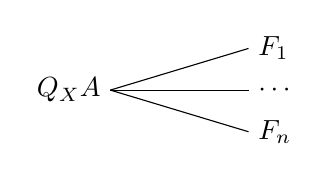
\begin{tikzpicture}
\tikzset{grow'=right}
%\tikzset{execute at begin node=\strut}
\tikzset{level distance=80pt}
\tikzset{every tree node/.style={align=left,anchor=west}}
\Tree [. $Q_XA$ $F_1$ $\cdots$ $F_n$ ]
\end{tikzpicture}
\end{center}
\noindent где $Q$ - некоторый квантор. Элементы дерева называются как обычно: \emph{узел}, \emph{корень}, \emph{лист}, \emph{ветвление}, и т.д. Поскольку $\forall$-кванторы соответствуют дизъюнкциям подформул $\{F_1,\ldots,F_n\}$ (кванторы $\exists$ соответствуют конъюнкции), тогда все $\forall$-узлы соответствуют {\em дизъюнктивному ветвлению}, а все $\exists$-узлы соответствуют {\em конъюнктивному ветвлению}.

Некоторые части канонической ПОФ будем называть следующим образом:
\begin{enumerate}
\item Корень ПОФ $\forall \varnothing$ называется {\em корнем} ПОФ.
\item Каждый непосредственный последователь $\exists_XA$ корня ПОФ называется {\em базой}, конъюнкт $A$ называется {\em базой фактов}, ПОФ, корнем которой является база называется {\em базовой подформулой}.
\item Каждый непосредственный последователь $\forall_YB$ базы ПОФ называется {\em вопросом} к своей базе. Если вопрос является листом дерева то он называется {\em целевым вопросом}.
\item Поддеревья вопросов называются {\em консеквентами}. Путая консеквента эквивалентна $\text{\textbf{False}}$.
\end{enumerate}

\begin{example}
Рассмотрим ПОФ представление некоторой ПЛФ.
$$F= \neg\bigl(\forall x\:\exists y P(x,y)\rightarrow \exists z P(z,z)\bigr).$$
Образом $F$ в языке ПОФ является $F' = \forall\colon \varnothing\{\exists\colon\varnothing\{\forall x\colon\varnothing\{\exists y\colon P(x,y)\}, \forall z\colon P(z,z)\{\exists\colon\boldsymbol{False}\}\}\}.$
А эта ПОФ в древовидной форме имеет следующий вид:
\begin{center}
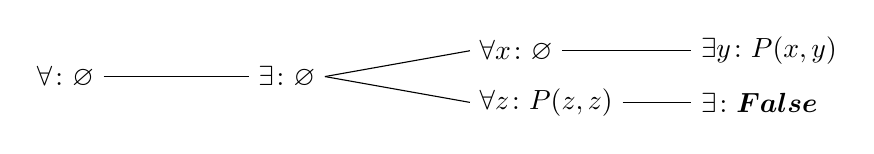
\begin{tikzpicture}
\tikzset{grow'=right}
%\tikzset{execute at begin node=\strut}
\tikzset{level distance=80pt}
\tikzset{every tree node/.style={align=left,anchor=west}}
\Tree [. $\forall\colon\varnothing$ [. $\exists\colon\varnothing$ [. $\forall x\colon\varnothing$ $\exists y\colon P(x,y)$ ] [. $\forall z\colon P(z,z)$ $\exists\colon\boldsymbol{False}$ ] ] ]
\end{tikzpicture}
\end{center}
\end{example}

\paragraph{Мотивация выбора средства разработки.}
Для систем АДТ важно затраченное время на решение задачи. Поскольку, разработанный транслятор (включая парсер) планируется использовать в системе АДТ для исчисления позитивно-образованных формул, эфективность трансляции тоже очень важна.

Эффективность работы программы в целом может зависить от двух факторов: 1) качество генерируемого кода компилятором (либо скорость исполнения интерпретатором); 2) качество используемых алгоритмов.

Для генерации эффективного кода необходимо использовать компилируемые языки, с нативной компиляцией. Наиболее известные из таких языков: С, С++, Pascal, FORTRAN, Rust и др. Кроме того, для них разработаны достаточно эффективные компиляторы. Мы будем использовать язык Rust. Особенность данного языка в том, что его компилятор генерирует код сопоставимый по скрости с компиляторами C и C++, но при этом в языке имеется ряд абстракций, позволяющий гарантировано избежать такие популярные ошибки как висячие указатели(Dangling pointer), дважды освобожденная память, инвалидирующий итератор и др. Кроме того в Rust имеется ряд конструкций, хорошо себя зарекомендовавших в функциональных языках, например, сопоставление с образом, лямбда-функции, функции высшего порядка и др.

%Разработка прувера, по вышеуказанным причинам ведется на языке Rust.
Для упрощения взаимодействия со структурами данных используемых в прувере, трансялтор также удобнее писать на Rust.

Синтаксический анализатор (парсер) является одним из основных составляющих транслятора. Есть два подхода к реализации парсеров: использовани генераторов парсеров; реализация вручную.

При первом подходе обычно используются такие средства как lex, yacc, antlr и тп. Это достаточно надежные программы, позволяющие упростить процесс создания парсера. Однако генерируемый ими код парсера может быть не так эффективен, а размер получаемого файла достаточно велик. Например, генератор LALRPOP для Rust, для грамматики TPTP создает файл размером порядка 1 миллиона строк.

Второй подход более сложен с точки зрения реализации, однако имеет преимущества перед первым подходом: эффективность кода может быть выше; размер файлов меньше; упрощается отлов ошибок.

\paragraph{Транслятор.}
Исходя из вышесказанного, мы выбрали второй подход. Нами используется классическая архитектура разбора грамматики: лексический анализ; затем синтаксический анализ.

Лексический анализатор реализован с помощью классического для данной задачи подхода - детерминированного конечного автомата (ДКА).

В качестве синтаксического анализа разработан LL1 парсер. Для этого грамматика TPTP была приведена к LL1 виду. Кроме того, грамматика TPTP была упрощена до вида, пригодного для парсинга только ПЛФ и КНФ, так как другие виды формул не предполагается поддерживать системой АДТ.

После стадии синтаксического анализа, наступает стадия трансляции исходной формулы (КНФ или ПЛФ) в ПОФ. %В целях повышения эффективности, некоторые этапы трансляции вынесены сразу на этап парсинга. %Но без значительного ущерба читаемости кода.

Результатом работы парсера является структура данных представляющая собой список аннотированных формул. В терминах библиотеки TPTP, такой список будем называть проблемой. Аннотированная формула имеет следующее поля: тип формулы (ПЛФ или КНФ); имя формулы, по которому можно, например, сослаться на данную формулу; роль формулы: аксиома, теорема, гипотеза и др. и, собственно, сама формула.

% \begin{enumerate}
% \item Шаг 1. Преобразование проблемы в ФПП. Полученная ФПП представляем собой отрицание конъюнкции всех формул, входящих в аннотированные формулы. Отриание производится с той целью, что прувер пытается опровергнуть трицание исходной формулы, чтоб тем самым подтвердить ее доказуемость. Полученную формулу будем называть исходной ФПП.

% \item Шаг 2. Удаление следующих связок: импликация, обратная импликация, эквиваленция с помощью правил Де Моргана, и проталкивание отрицаний до атомарных формул.

% \item Шаг 3. Формула типа FolFormula преобразуется в тип XFolFormula. На данном шаге все строковые имена переменных, констант и функторов заменяются на числовые коды. Строится таблица символов, в которой каждому коду дано соответствующее ему строкове представлеие. Во-первых, это делается для повышения эффективности дальнейшей работы с формулой, так как операции сравнения целых чисел производятся намного быстрее чем операции сравнения строк, кроме того числовые значения занимают меньше памяти. Во-вторых, такой подход позволяет различать переменные с одинаковым строковым представлением, но управляемые разными квантоами. Например в формуле Foral(X,Y): a(X,Y) and Forall(Y): b(Y). Первое вхождение Y управляется первым квантором, а второе вторым. Числовой код будет дан разный. Этим занимается процедура prepfof.

% \item Шаг 4. Уплощение дизъюнкций и конъюнкций. Для

% Например, если есть формула A and B and (C and E), то она преобразуется в A and B and C and E.

% \item Шаг 5. Построение первой версии ПОФ. Алгоритм

% \item Шаг 6. В полученной формуле делаем редукцию фиктивных универсальных квантором не имеющих дизъюнктивного ветвления. Данный шаг можно отнести уже к процедуре логического вывода, однако он выполняется на этапе трансляции, чтобы не захламлять по-формулы фиктивными кванторами. Кванторы с дизветвлением не редуцируются, поскольку они потенциально приводят к увеличению количества узлов формулы. Данный вопрос уже разрешается системой логического вывода (прувером). Пожалуй описать можно как применение правила вывода омега к фикивным а-кванторам.

% \item Шаг 7. Делаем редукцию фиктивных е-кванторов.

% \end{enumerate}

%=======================================================
%=======================================================
%=======================================================
%Шаг 1

Важными характеристиками полученной в результате трансляции ПОФ являются: 1) Количество узлов в древовидном представлении ПОФ. 2) Количество фиктивных кванторов. Поэтому процедура трансляции ПЛФ в ПОФ состоит из нескольких шагов, часть из которых направлены на уменьшение количества узлов и уменьшение количства фиктивных кванторов. Исходная эвристическая структура формулы ПЛФ, сохраняется благодаря тому, что сохраняется исходный порядок следования кванторов $\forall$ и $\exists$, в отличии от процедуры скулемизации, используемой для получения КНФ, устраняющей кванторы $\exists$ и вносящей в формулу дополнительные термы.

\paragraph{Описание шагов метода трансляции.}

Метод трансляции состоит из следующих шагов.

\textbf{Шаг 1.} Преобразование проблемы в ПЛФ. Полученная ПЛФ представляем собой отрицание конъюнкции всех формул, входящих в аннотированные формулы. Отрицание производится с той целью, что система АДТ опровергает отрицание исходной формулы, чтоб тем самым подтвердить ее доказуемость. %Полученную формулу будем называть исходной ФПП.

%=======================================================
%=======================================================
%=======================================================
%Шаг 2
\textbf{Шаг 2.} Удаление связок $\leftrightarrow$, $\rightarrow$, снятие двойного отрицания и приминение законов де Моргана. Пусть $F$, возможно с индексом, произвольная неатомарная ПЛФ, а $A$ - атомарная ПЛФ. Тогда правила преобразований (назовем эту группу преобразований $\pi_0$) представлены в таблице 1.

\begin{table}[htbp]
	\caption{Правила преобразований $\pi_0$}\vspace*{2mm}

	\begin{tabular}{|l|l|}
		\hline
		\textbf{Исходная формула} & \textbf{Результирующая формула} \\
		\hline
		$\neg\neg F$ & $F^{\pi_0}$ \\

		\hline
		$\neg (F_1 \rightarrow F_2)$ & ${F_1}^{\pi_0} \& {\neg F_2}^{\pi_0}$ \\

		\hline
		$\neg (F_1 \leftrightarrow F_2)$ & $(\neg(F_1 \rightarrow F_2))^{\pi_0} \vee (\neg(F_2 \rightarrow F_1))^{\pi_0}$ \\

		\hline
		$\neg (F_1 \&\ldots\& F_n)$ & $(\neg F_1)^{\pi_0} \vee\ldots\vee (\neg F_n)^{\pi_0}$ \\

		\hline
		$\neg (F_1 \vee\ldots\vee F_n)$ & $(\neg F_1)^{\pi_0} \&\ldots\& (\neg F_n)^{\pi_0}$ \\

		\hline
		$\neg\forall{x}F$ & $\exists{x}(\neg F)^{\pi_0}$ \\

		\hline
		$\neg\exists{x}F$ & $\forall{x}(\neg F)^{\pi_0}$ \\

		\hline
		$\neg A$ & $\neg A$ \\

		\hline
		$F_1 \rightarrow F_2$ & $(\neg F_1)^{\pi_0} \vee {F_2}^{\pi_0}$ \\

		\hline
		$F_1 \leftrightarrow F_2$ & $(\neg F_1 \vee F_2)^{\pi_0} \& (\neg F_2 \vee F_1)^{\pi_0} $ \\

		\hline
		$F_1 \&\ldots\& F_n$ & ${F_1}^{\pi_0} \&\ldots\& {F_n}^{\pi_0} $ \\

		\hline
		$F_1 \vee\ldots\vee F_n$ & ${F_1}^{\pi_0} \vee\ldots\vee {F_n}^{\pi_0} $ \\

		\hline
		$\forall{x}F$ & $\forall{x}(F)^{\pi_0} $ \\

		\hline
		$\exists{x}F$ & $\exists{x}(F)^{\pi_0} $ \\

		\hline
	\end{tabular}
\end{table}

%=======================================================
%=======================================================
%=======================================================


%=======================================================
%=======================================================
%=======================================================
% Шаг 4
\textbf{Шаг 3.} Уплощение конъюнкций и дизъюнкций

Пусть $\circ \in\{\vee,\&\}$. Правило уплощения дизъюнкций и конъюнкций $flat$:

Пусть $F = G_1 \circ \ldots \circ G_n \circ C_1 \circ\ldots\circ C_m$, где $C_i = (C_{i1} \circ\ldots\circ C_{ik_i})$, тогда $$F^{flat} = G_1 \circ\ldots\circ G_n \& C_{11} \circ\ldots\circ C_{1k_1} \circ \ldots \circ C_{m1} \circ\ldots\circ C_{mk_m}$$

Смысл названия уплощение хорошо виден, если формулу представить синатксическим деревом. Например, следующие представления эквивалентны:

\Tree[. $\forall x$ [. $\&$ $F_1$ [. $\&$ $G_1$ $G_2$ ] $F_2$  ] ]
и
\Tree[. $\forall x$ [. $\&$ $F_1$ $G_1$ $G_2$ $F_2$  ] ]

%=======================================================
%=======================================================
%======================================================
% Шаг 5

\textbf{Шаг 4.} Трансляция ПЛФ в ПОФ. Пусть $G$, возможно с индексами, есть некоторая ПЛФ, а $A$, возможно с индексами, атомарная ПЛФ.

Введем еще одно обозначение. Пусть $P,Q\in\{\forall,\exists\}, P\neq Q$, $C$ - некоторый конъюнкт, тогда:
\begin{displaymath}
\begin{array}{l}
%A=A^{\&} = \bigand{n}{i=1}A_i(t_1,\ldots,t_k)\\
F^Q = \left\lbrace
		  \begin{array}{l}
		  F, \text{если } F = Q_X\colon C \;\Phi,\\
		  Q\colon\varnothing(F), \text{если } F = P_X\colon C \;\Phi,
		  \end{array}\right.

\end{array}
\end{displaymath}

Тогда правила преобразования $\pi_1$ представлены в таблице 2.

Правило уплощения позволяет ограничить, насколько это возможно, применение правил 13 и 14, которые приводят к необязательному появлению фиктивных кванторов.

\begin{table}[htbp]
	\caption{Правила преобразований $\pi_1$}\vspace*{2mm}
	%\centering \small\label{tabl_1}

	\begin{tabular}{|l|l|l|}
		\hline
		\textbf{№} & \textbf{ПЛФ} & \textbf{ПО-формула} \\
		\hline
		1 & $\exists{x}\exists{y}G$ & $(\exists{x,y}G)^{\pi_1}$ \\
		\hline
		2 & $\exists{x}\forall{y}G$ & $\exists{x}\colon\varnothing(\forall{y}G)^{\pi_1}$ \\
		\hline
		3 & $\exists{x}G_1 \& \ldots \& G_n \& A_1 \& \ldots \& A_m $ & $\exists{x}\colon A_1 \& \ldots \& A_m ((G_{1}^{\pi_1})^{\forall},\ldots,(G_{n}^{\pi_1})^{\forall})$ \\
		\hline
		4 & $\exists{x}G_1 \vee \ldots \vee G_n \vee \neg A_1 \vee \ldots \vee \neg A_m$ & $\exists{x}\colon\varnothing \forall\colon A_1 \& \ldots \& A_m (G_{1}^{\pi_1})^{\exists},\ldots,(G_{n}^{\pi_1})^{\exists}$ \\
		\hline
		5 & $\exists{x}\neg A$ & $\exists{x}\colon\varnothing(\forall\colon A)$  \\
		\hline
		6 & $\exists{x}A$ & $\exists{x}\colon A$ \\
		\hline
		7 & $\forall{x}\exists{y}G$ & $\forall{x}\colon\varnothing(\exists{y}G)^{\pi_1}$ \\
		\hline
		8 & $\forall{x}\forall{y}G$ & $(\forall{x,y}G)^{\pi_1}$ \\
		\hline
		9 & $\forall{x}G_1 \& \ldots \& G_n \& A_1 \& \ldots \& A_m$ & $\forall{x}\colon\varnothing \exists\colon A_1 \& \ldots \& A_m (G_{1}^{\pi_1})^{\forall},\ldots,(G_{n}^{\pi_1})^{\forall}$ \\
		\hline
		10 & $\forall{x}G_1 \vee \ldots \vee G_n \vee \neg A_1 \vee \ldots \vee \neg A_m$ & $\forall{x}\colon A_1 \& \ldots \& A_m (G_{1}^{\pi_1})^{\exists},\ldots,(G_{n}^{\pi_1})^{\exists}$ \\
		\hline
		11 & $\forall{x}\neg A$ & $\forall{x}\colon A$ \\
		\hline
		12 & $\forall{x}A$ & $\forall{x}\colon\varnothing (\exists\colon A)$ \\
		\hline
		13 & $G_1 \&\ldots\& G_n$ & $\exists\colon\varnothing({G_1}^{\pi_1})^{\forall},\ldots,({G_n}^{\pi_1})^{\forall}$ \\
		\hline
		14 & $G_1 \vee\ldots\vee G_n$ & $\forall\colon\varnothing({G_1}^{\pi_1})^{\exists},\ldots,({G_n}^{\pi_1})^{\exists}$ \\
		\hline
		15 & $\neg A$ & $\forall \colon A$ \\
		\hline
		16 & $A$ & $\exists \colon A$ \\
		\hline
	\end{tabular}
\end{table}

%=======================================================
%=======================================================
%=======================================================
%\if 0
\textbf{Шаг 5. (Правило сокращения)}

В получаемой формуле возникают узлы с фиктивными кванторами $\forall\varnothing$ и $\exists\varnothing$, кроме этого, могут возникнуть излишние ветвления, плохо влияющие на дальнейший поиск вывода. Следующее правило позволяет максимально сократить получаемое дерево.

Если в некоторой ПО-формуле $F$:
\begin{center}
	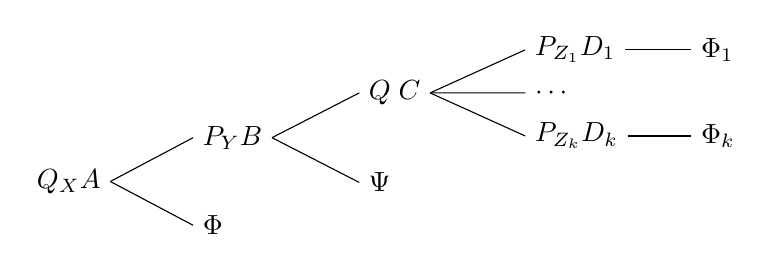
\begin{tikzpicture}
	\tikzset{grow'=right}
	%\tikzset{execute at begin node=\strut}
	\tikzset{level distance=60pt}
	\tikzset{every tree node/.style={align=left,anchor=west}}
	\Tree [. $Q_{X}A$ [. $P_{Y}B$ [. $Q\;C$ [. $P_{Z_1}D_1$ $\Phi_1$ ] $\cdots$ [. $P_{Z_k}D_k$ $\Phi_k$ ] ] $\Psi$ ] $\Phi$ ]
	\end{tikzpicture}
\end{center}
$P,Q\in\{\forall,\exists\}, P\neq Q$, $C,B$ - конъюнкты, удовлетворяющие условию $C\subseteq B$, то $F$ эквивалентна $F'$ имеющей следующий вид:

\begin{center}
	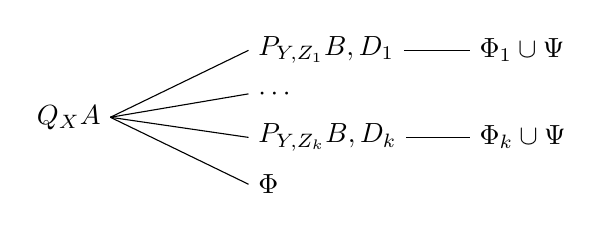
\begin{tikzpicture}
	\tikzset{grow'=right}
	%\tikzset{execute at begin node=\strut}
	\tikzset{level distance=80pt}
	\tikzset{every tree node/.style={align=left,anchor=west}}
	\Tree [. $Q_{X}A$ [. $P_{Y,Z_1}B,D_1$ $\Phi_1\cup\Psi$ ] $\cdots$ [. $P_{Y,Z_k}B,D_k$ $\Phi_k\cup\Psi$ ] $\Phi$ ]
	\end{tikzpicture}
\end{center}

Представленное правило нуждается в доказательстве.

Пусть конъюнкт $C$ имеет вид $C^1\&\ldots\& C^n$. Если $C\subseteq B$, то $B = B'\&C^1\&\ldots\& C^n$, где $B'$ некоторый, возможно пустой конъюнкт. Переведем ПО-формулу $F$ в язык исчисления предикатов. В случае, если $F$ начинается с квантора $\forall$:
$$F = \forall_X A\rightarrow\bigl(\Phi\vee\exists_Y(\Psi\& B\&(\neg C\vee\exists_{Z_1}(D_1\&\Phi_1)\vee\ldots\vee\exists_{Z_k}(D_k\&\Phi_k)))\bigr)$$
При раскрытии скобок получаем дизъюнкицию конъюнкций, одна из которых: $\Psi\&B\&\neg C = (\Psi\&B'\&C^1\&\ldots\& C^n)\&(\neg C^1\vee\ldots\vee C^n) = \text{\textbf{False}}$, т.е. является несущественной. Поэтому
$$F = \forall_X A\rightarrow\bigl(\Phi\vee\exists_Y\exists_{Z_1}(B\&D_1\&\Psi\&\Phi_1)\vee\ldots\vee\exists_Y\exists_{Z_k}(B\&D_k\&\Psi\&\Phi_k))\bigr),$$
что при переводе в ПОФ-представление имеет вид совпадающий с $F'$.

Если $F$ начинается с квантора $\exists$, после перевода в язык исчисления предикатов получаем:
$$F = \exists_X A\&\Phi\&(\forall_Y B\rightarrow (\Psi\vee C\&\forall_{Z_1}(D_1\rightarrow\Phi_1)\&\ldots\&\forall_{Z_k}(D_k\rightarrow\Phi_k))).$$
Распишем выражение в скобке:
$$\forall_Y B\rightarrow (\Psi\vee C\&\forall_{Z_1}(D_1\rightarrow\Phi_1)\&\ldots\&\forall_{Z_k}(D_k\rightarrow\Phi_k))$$
Устраняем импликацию и группируем дизъюнктивные элементы в отдельную скобку.
$$\forall_Y ((\neg B'\vee\neg C^1\vee\ldots\vee\neg C^n\vee\Psi) \vee C^1\&\ldots\& C^n\&\forall_{Z_1}(D_1\rightarrow\Phi_1)\&\ldots\&\forall_{Z_k}(D_k\rightarrow\Phi_k)).$$
Применяяя закон дистрибутивности, получаем:
$$\forall_Y ((\neg B'\vee\neg C^1\vee\ldots\vee\neg C^n\vee\Psi\vee C^1)\&\ldots\&(\neg B'\vee\neg C^1\vee\ldots\vee\neg C^n\vee\Psi\vee C^n)\&$$
$$(\neg B'\vee\neg C^1\vee\ldots\vee\neg C^n\vee\Psi\vee\forall_{Z_1}(D_1\rightarrow\Phi_1) )\&\ldots\&$$
$$(\neg B'\vee\neg C^1\vee\ldots\vee\neg C^n\vee\Psi\vee\forall_{Z_k}(D_k\rightarrow\Phi_k) )).$$
В первых $n$ скобках присутствует тавтология $\neg C^i\vee C^i$, поэтому:
$$\forall_Y (\text{\textbf{True}}\&\ldots\&\text{\textbf{True}}\&(\neg B\vee\Psi\vee\forall_{Z_1}(D_1\rightarrow\Phi_1) )\&\ldots\&(\neg B\vee\Psi\vee\forall_{Z_k}(D_k\rightarrow\Phi_k) )) = $$
$$\forall_Y\forall_{Z_1}(\neg(B\& D_1)\vee\Psi\vee\Phi_1)\&\ldots\&\forall_Y\forall_{Z_k}(\neg(B\& D_k)\vee\Psi\vee\Phi_k).$$
Т.е. $$F = \exists_X A\&\Phi\&\forall_Y\forall_{Z_1}((B\& D_1)\rightarrow(\Psi\vee\Phi_1))\&\ldots\&\forall_Y\forall_{Z_k}((B\& D_k)\rightarrow(\Psi\vee\Phi_k)),$$
что при переводе в ПОФ-представление имеет вид совпадающий с $F'$.

Доказательство завершено.

%\fi

\if 0
\textbf{Шаг 6.} Редукция фиктивных $\forall$-кванторов, не имеющих дизъюнктивного ветвления. Правило $\pi_2$
Если
$F = \forall{x}\colon C F_1,\ldots,F_n$

Тогда
$F^{\pi_2} = \forall{x}\colon C {F_1}^{\pi_2},\ldots,{F_n}^{\pi_2}$

Если
$F = \exists{x}\colon C F_1,\ldots,F_n, D_1,\ldots,D_m$, где $F_i = \forall{y}\colon C_i G_{i1},\ldots,G_{ij}$, $j > 1$ и $D_i = \forall\colon\varnothing\exists{z_i}\colon E_i P_{i1},\ldots P_{ik}$. Иными словами, формулы  $F_i$ имеют дизъюнктивное ветвление, а $D_i$ не имеют и являются фиктивными. И тех и тех формул может быть $0$.

Тогда
$F^{\pi_2} = \exists{x \cup z_1 \cup\ldots\cup z_m}\colon {C \cup E_1 \cup\ldots\cup E_m} {F_1}^{\pi_2},\ldots,{F_n}^{\pi_2},P_{11}^{\pi_2},\ldots,P_{mk}^{\pi_2}$

\textbf{Шаг 7.} Редукция фиктивных $\exists$-кванторов, не имеюших ветвления. Правило $\pi_3$

Если
$F = \exists{x}\colon C F_1,\ldots,F_n$

Тогда
$F^{\pi_3} = \exists{x}\colon C {F_1}^{\pi_3},\ldots,{F_n}^{\pi_3}$

Если
$F = \forall{x}\colon C F_1,\ldots,F_n,G_1,\ldots,G_m$, где $F_i$ - $\exists$-формула, с нефиктивнм квантором в корне, а $G_i = \exists\colon\forall{y_i}\colon A_i E_{i1},\ldots,E_{ik}$

Тогда

$F^{\pi_3} = \forall{x \cup y_1 \cup\ldots\cup y_m}\colon C \cup A_1 \cup\ldots\cup A_m E_{11}^{\pi_3},\ldots,E_{mk}^{\pi_3},{F_1}^{\pi_3},\ldots,{F_n}^{\pi_3}$

\fi

В библиотеке TPTP, кроме задач в общем классическом первопорядковом представлении, достаточно большое количество задач представлено в виде множеств дизъюнктов, задачи приведены к скулемовской стандартной форме и восстановить первоначальную формализацию таких задач проблематично. Для перевода задач представленных в виде множеств дизъюнктов, в которых отсутствуют переменные связанные кванторами существования, достаточно воспользоваться нижеприведенной формулой. Объединим дизъюнкты некоторого множества $S$ в классы $C^1$, $C^2$, $C^3$, $C^4$, которые определяются следующим образом:

\begin{enumerate}
	\item $C^1 = \{ C^{1}_{1},\ldots, C^{1}_{n_1} \}$ - множество единичных основных (не содержащих переменных) положительных дизъюнктов;
	\item $C^2 = \{ C^{2}_{1},\ldots, C^{2}_{n_2} \}$ - множество положительных дизъюнктов, т.е. $C^{2}_{j} = \bigvee^{k_j}_{i=1} L^{2_j}_i$, $\forall j=\overline{1,n_2}$, где $L^{2_j}_i$ - положительные литеры, $k_j>1$ - количество литер в соответствующих дизъюнктах, обозначим через $X^2_j$ - множество переменных, встречающихся в дизъюнкте $C^2_j$;
	\item $C^3 = \{ C^{3}_{1},\ldots, C^{3}_{n_3} \}$ - множество отрицательных дизъюнктов, т.е. $C^{3}_{j} = \bigvee^{k_j}_{i=1}\neg L^{3_j}_i$, $\forall j=\overline{1,n_3}$, где $^{3_j}L_i$ - положительные литеры, $k_j>1$ - количество литер в соответствующих дизъюнктах, обозначим через $X^3_j$ - множество переменных, встречающихся в дизъюнкте $C^3_j$;
	\item $C^4 = \{ C^{4}_{1},\ldots, C^{4}_{n_4} \}$ - множество дизъюнктов, содержащих и положительные, и отрицательные литеры, т.е. $C^{4}_{j} = \bigvee^{m_j}_{i=1}\neg L^{4_j}_i\vee\bigvee^{k_j}_{i=m_{j}+1}L^{4_j}_i$, $\forall j=\overline{1,n_4}$, где $L^{4_j}_i$ - положительные литеры, $m_j>0, k_j>0$ - количество отрицательных и положительных литер в соответствующих дизъюнктах, обозначим через $X^4_j$ - множество переменных, встречающихся в дизъюнкте $C^4_j$;
\end{enumerate}

ПО-формула, соответствующая упорядоченному таким образом множеству дизъюнктов будет иметь вид:

\begin{center}
	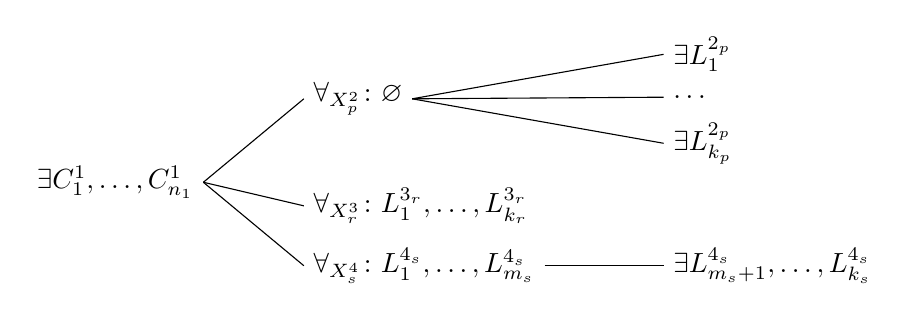
\begin{tikzpicture}
	\tikzset{grow'=right}
	%\tikzset{execute at begin node=\strut}
	%\tikzset{level distance=70pt}
	\tikzset{level 1/.style={level distance=100pt}}
	\tikzset{level 2/.style={level distance=130pt}}
	\tikzset{level 3+/.style={level distance=50pt}}
	\tikzset{every tree node/.style={align=left,anchor=west}}
	\Tree [. $\exists C^{1}_{1},\ldots,C^{1}_{n_1}$ [. $\forall_{X^{2}_{p}}\colon\varnothing$ $\exists L_{1}^{2_p}$ $\ldots$ $\exists L_{k_{p}}^{2_p}$ ] $\forall_{X^{3}_{r}}\colon L^{3_r}_{1},\ldots,L^{3_r}_{k_r}$ [. $\forall_{X^{4}_{s}}\colon L^{4_s}_{1},\ldots,L^{4_s}_{m_s}$ $\exists L^{4_s}_{m_{s}+1},\ldots,L^{4_s}_{k_{s}}$ ] ]
	\end{tikzpicture}
\end{center}

\noindent
$\forall p=\overline{1,n_2}, \forall r=\overline{1,n_3}, \forall s=\overline{1,n_4}$. Поэтому итоговая формула будет содержать $n_2$ подформул соответствующих дизъюнктам класса $C^2$, $n_3$ подформул - класса $C^3$ и $n_4$ подформул - класса $C^4$.

%=======================================================
%=======================================================
%=======================================================



%=======================================================
%=======================================================
%=======================================================



\paragraph{Тестирование.}

Тестирование алгоритмов транслирования производилось на задачах из библиотеки ТПТП. Использовался компьютер MacBook Pro с процессором 2,3 GHz Intel Core i7 и оперативной памятью 8 GB 1600 MHz DDR3.

Всего было отобрано 6817 задач. Была собрана некоторая статистика. Количество задач, для которых ПЛФ представление содержит меньше узлов чем ПОФ представление: 1169.
%Среднее соотношение поф/фоф: 1.31041311391
%Коэффициент вариации: 0.199877542518
%
Количество задач, для которых ПОФ представление содержит меньше узлов чем ПЛФ представление: 5648.
Корреляция между количеством узлов в ПЛФ и количеством узлов в соответствующей ПОФ равна 0.77.

Корреляция между количеством неограниченных переменных в ПОФ и рейтингом задачи в библиотеке ТПТП равна 0.2. Данный факт, говорит о том, что для систем АДТ, основанных на методе резолюций, не имеет значения содержит ли формализация задачи неограниченные переменные. Однако, для метода АДТ основанном на ПОФ-исчислении, отсутствие неограниченных переменных заметно улушает эффективность поиска логического вывода. Поэтому, с помощью ПОФ-исчисления естественным образом выделяется особый класс формул, которые решаются эффективнее чем методом резолюций.


%Среднее соотношение фоф/поф: 362.38103709

%Коэффициент вариации: 44.0850467178

%
%Когда в фоф меньше связок чем узлов в поф: 2488

%Среднее соотношение поф/фоф: 1.6170763397

%Коэффициент вариации: 0.324110418939

%
%Когда в поф меньше узлов чем связок в фоф: 2975

%Среднее соотношение фоф/поф: 1.68320625411

%Коэффициент вариации: 0.448233170066


\begin{table}[htbp]
	\caption{Задачи, когда узлов в ПОФ больше чем в 2 раза чем в ПЛФ}\vspace*{2mm}
	\begin{tabular}{|l|l|l|l|l|}
		\hline
		\textbf{ТПТП} & \textbf{Узлов в ПЛФ} & \textbf{Связок в ПЛФ} & \textbf{Узлов в ПОФ} & \textbf{Время секунд} \\
		\hline
		HWV097+1.p & 66290 & 57069 & 136382 & 0.540536885 \\
		\hline
		LCL181+1.p & 6 & 5 & 13 & 0.001467201 \\
		\hline
		SET047+1.p & 8 & 4 & 23 & 0.000362342 \\
		\hline
		SET194+3.p & 20 & 11 & 41 & 0.000434487 \\
		\hline
		SET577+3.p & 28 & 17 & 57 & 0.000504854 \\
		\hline
		SET580+3.p & 25 & 16 & 55 & 0.000482766 \\
		\hline
		SET624+3.p & 23 & 14 & 47 & 0.000475778 \\
		\hline
		SET788+1.p & 8 & 4 & 22 & 0.000393746 \\
		\hline
		SEU142+1.p & 26 & 16 & 54 & 0.000589682 \\
		\hline
		SEU149+1.p & 22 & 14 & 46 & 0.000621684 \\
		\hline
	\end{tabular}
\end{table}


\begin{table}[htbp]
	\caption{Задачи, когда узлов в ПЛФ больше чем в 5 раза чем в ПОФ}\vspace*{2mm}
	\begin{tabular}{|l|l|l|l|l|}
		\hline
		\textbf{ТПТП} & \textbf{Узлов в ПЛФ} & \textbf{Связок в ПЛФ} & \textbf{Узлов в ПОФ} & \textbf{Время секунд} \\
		\hline
		AGT024+2.p & 1105 & 1071 & 182 & 0.014771418 \\
		\hline
		AGT025+2.p & 1105 & 1071 & 182 & 0.012581508 \\
		\hline
		AGT026+2.p & 1105 & 1071 & 182 & 0.013624296 \\
		\hline
		GEO301+1.p & 2603 & 2077 & 516 & 0.014960987 \\
		\hline
		GEO302+1.p & 2604 & 2078 & 516 & 0.015018181 \\
		\hline
		GEO303+1.p & 2605 & 2079 & 516 & 0.015902619 \\
		\hline
		GRA026+1.p & 66 & 60 & 12 & 0.00066178 \\
		\hline
		LCL648+1.001.p & 16 & 12 & 2 & 0.000773028 \\
		\hline
		LCL649+1.001.p & 17 & 13 & 3 & 0.001689769 \\
		\hline

	\end{tabular}
\end{table}


\begin{table}[htbp]
	\caption{Наиболее трудоемкие для транляции задачи}\vspace*{2mm}
	\begin{tabular}{|l|l|l|l|l|}
		\hline
		\textbf{ТПТП} & \textbf{Узлов в ПЛФ} & \textbf{Связок в ПЛФ} & \textbf{Узлов в ПОФ} & \textbf{Время секунд} \\
		\hline
		HWV067+1.p & 356879.0 & 356875.0 & 209006.0 & 25.676720753 \\
		\hline
		HWV061+1.p & 492486.0 & 492482.0 & 251387.0 & 20.676587109 \\
		\hline
		HWV134+1.p & 2143011.0 & 2001596.0 & 4176067.0 & 19.714228823 \\
		\hline
		HWV133+1.p & 2141861.0 & 2000646.0 & 4174817.0 & 19.680084771 \\
		\hline
		HWV132+1.p & 2141171.0 & 2000076.0 & 4174067.0 & 19.527616096 \\
		\hline
		HWV064+1.p & 271751.0 & 271747.0 & 171054.0 & 18.413976178 \\
		\hline
		HWV063+1.p & 271751.0 & 271747.0 & 171054.0 & 18.13921648 \\
		\hline
		HWV068+1.p & 204095.0 & 204091.0 & 115846.0 & 10.485964562 \\
		\hline
		HWV100+1.p & 837934.0 & 752470.0 & 1624765.0 & 7.2706892 \\
		\hline
		HWV092+1.p & 832887.0 & 747414.0 & 1615877.0 & 7.258642311 \\
		\hline
		SEU418+4.p & 831581.0 & 655928.0 & 391496.0 & 6.787772546 \\
		\hline
		SEU423+4.p & 831659.0 & 655980.0 & 391541.0 & 6.540693459 \\
		\hline
		SEU422+4.p & 831641.0 & 655967.0 & 391529.0 & 6.477316638 \\
		\hline
		SEU419+4.p & 831605.0 & 655943.0 & 391510.0 & 6.335897181 \\
		\hline
		HWV126+1.p & 794534.0 & 582596.0 & 1445841.0 & 6.315884604 \\
		\hline
		HWV128+1.p & 794774.0 & 582836.0 & 1445921.0 & 6.285583186 \\
		\hline

	\end{tabular}
\end{table}
%%%%%%%%% Вставка рисунка %%%%%%%%%%%%%

% \begin{figure}[htbp]
%     \centering
% %\includegraphics[width=85mm]{Pic1.eps}
% %\includegraphics[width=40mm]{fig1.png}
% \includegraphics[width=70mm]{ris1.pdf}
% \caption{<Подрисуночная подпись>}
% \end{figure}

%%%%%%%%% Вставка таблицы %%%%%%%%%%%%%

% \begin{table}[htbp]
% \caption{Заголовок таблицы}\vspace*{2mm}
% \centering \small\label{tabl_1}

% \begin{tabular}{c|c|c|c}
% %\hline
% %\multicolumn{2}{c||}{Сетка}  & \multicolumn{2}{c}{} \\
% % \cline{2-4}
% \hline
% $i$ & $N_1\times N_2$ & $R_i$ & $R_{i-1}/R_i$ \\
% \hline
% 1& $20\times20$ & $7.2\cdot10^{-4}$ &  --- \\
% \hline
% 2& $40\times40$ & $9.9\cdot10^{-5}$ & 7.3 \\
% \hline
% 3& $80\times80$ & $1.4\cdot10^{-5}$ & 7.1 \\
% \hline
% 4& $160\times160$ & $1.7\cdot10^{-6}$ & 8.2\\
% \end{tabular}
% \end{table}

%\paragraph{Благодарности.} Работа выполнена при финансовой поддержке РФФИ (грант \No~...) и др.

\paragraph{Заключение.}

В работе приводится краткое описание языка позитивно-образованных формул и рассматриваются вопросы обработки ПОФ перед запуском автоматических алгоритмов поиска вывода. Представлен метод преобразования первопорядковых логических формул в язык ПОФ в виде эффективных алгоритмов обработки первопорядковых формул. Разработанные алгоритмы сохраняют исходную эвристическую структуру знаний представленных формулами языка исчисления предикатов. Рассмотрены вопросы преобразования формул языка дизъюнктов в язык ПОФ и предложен упрощенный алгоритм для трансляции таких задач. Приводятся результаты тестирования разработанного метода на задачах из библиотеки TPTP. Была собрана некоторая статистика из которой следует, что помощью ПОФ-исчисления естественным образом выделяется особый класс формул, которые решаются эффективнее чем методом резолюций.


\begin{thebibliography}{9}

\bibitem{SNV1990} {\sc Vassilyev~S.N.}
Machine Synthesis of Mathematical Theorems // The Journal of Logic programming.~--- 1990. V.9~--- No.2--3.~--- pp.~235--266.

\bibitem{ICDS2000} {\sc Васильев~С.Н., Жерлов~А.К., Федунов~Е.А., Федосов~Б.Е.}
Интеллектное управление динамическими системами~/ Москва: ФИЗМАТЛИТ, 2000. ---352~c.

\bibitem{jour2} {\sc Davydov~A.V., Larionov~A.A., Cherkashin~E.A.}
On the calculus of positively constructed formulas for automated theorem proving // Automatic Control and Computer Sciences (AC\&CS).~--- 2011.~--- V.45.~--- No.7.~--- pp. 402--407.

\bibitem{Cherkashin}
{\sc Черкашин Е.А.} Программная система «Квант/1» для автоматического доказательства теорем. --- канд. дисс. Текст. ИДСТУ СО РАН, Иркутск, 1999.

\bibitem{mipro2013} {\sc Cherkashin~E.A., Davydov~A.V., Larionov~A.A.}
Calculus of Positively Constructed Formulas, its Features, Strategies and Implementation // MIPRO 2013/CIS (36-th international convention on information and communication technology, electronics and microelectronics), 20-24 May 2013, Chroatia, Opatija.~--- 2013.~--- pp. 1289--1295.

\bibitem{tptp} {\sc Sutcliffe~G.}
The TPTP Problem Library and Associated Infrastructure. The FOF and CNF Parts, v3.5.0 // Journal of Automated Reasoning.~---2009.~--- V43.~--- N4.~--- pp.337--362.

\bibitem{SMTtoTPTP} {\sc Baumgartner~P.}
SMTtoTPTP -- A Converter for Theorem Proving Formats // In book: Felty~P.~A, Middeldorp~A., editors, "Automated Deduction - CADE-25: 25th International Conference on Automated Deduction, Berlin, Germany, August 1-7, 2015, Proceedings"~/~Cham:Springer International Publishing,~---2015.~pp.285--294.

\bibitem{Bourbaki} {\sc Bourbaki~N.}
Theory of Sets~/ Paris: Hermann, 1968.

\end{thebibliography}


%%%%%%%%% Ниже дается англоязычная часть %%%%%%%%%
\if 0
\begin{abstract}
	{
		%\en
		\noindent
		\begin{flushleft}
			\textbf{<Title>\let\thefootnote\relax\footnote{\copyright\ ICT SB RAS, 2016}}\\[1em]
			{\sc Ivanov, Ivan I.$^{1,*}$, Ivanova, Irina I.$^2$ ...}\\[.5em]
			$^1$\vtop{\footnotesize  Institute of Computational Technologies SB RAS, Novosibirsk, 630090, Russia}\\
			$^2$\vtop{\footnotesize  Novosibirsk State University, Novosibirsk, 630090, Russia}\\[.2em]
			$^*$\vtop{\footnotesize Corresponding author:  Ivanov, Ivan I.,  e-mail: \tt ...}\\[1em]
		\end{flushleft}


		<Abstract (200--250 слов)>\\


		<\textit{Keywords}:>

		\paragraph{\small Acknowledgements.}  This research was partly supported by RFBR (grant No.~...) et al.

		\vspace*{5.mm}

		%{\footnotesize\it \hfill Received  5 October 2015
		%
		%\hfill Received in revised form 3 December 2015}

		\hfill}
\end{abstract}

\fi

\end{document}
